\chapter{Implementation}
\label{chapter6}

\section{Development Environment}
The development of this project was done in various environments, as there was many different aspects to this project.

\subsection{Vive Hardware}
For this project, the Vive Hardware was set up in a dedicated room (The Virtual Reality Lab in the School of Computing). This allowed development to be done on the HTC Vive without having to set up the sensors and calibrate the hardware every time that development had to be done, which maximised the amount of development time that was available.

\begin{figure}[H]
	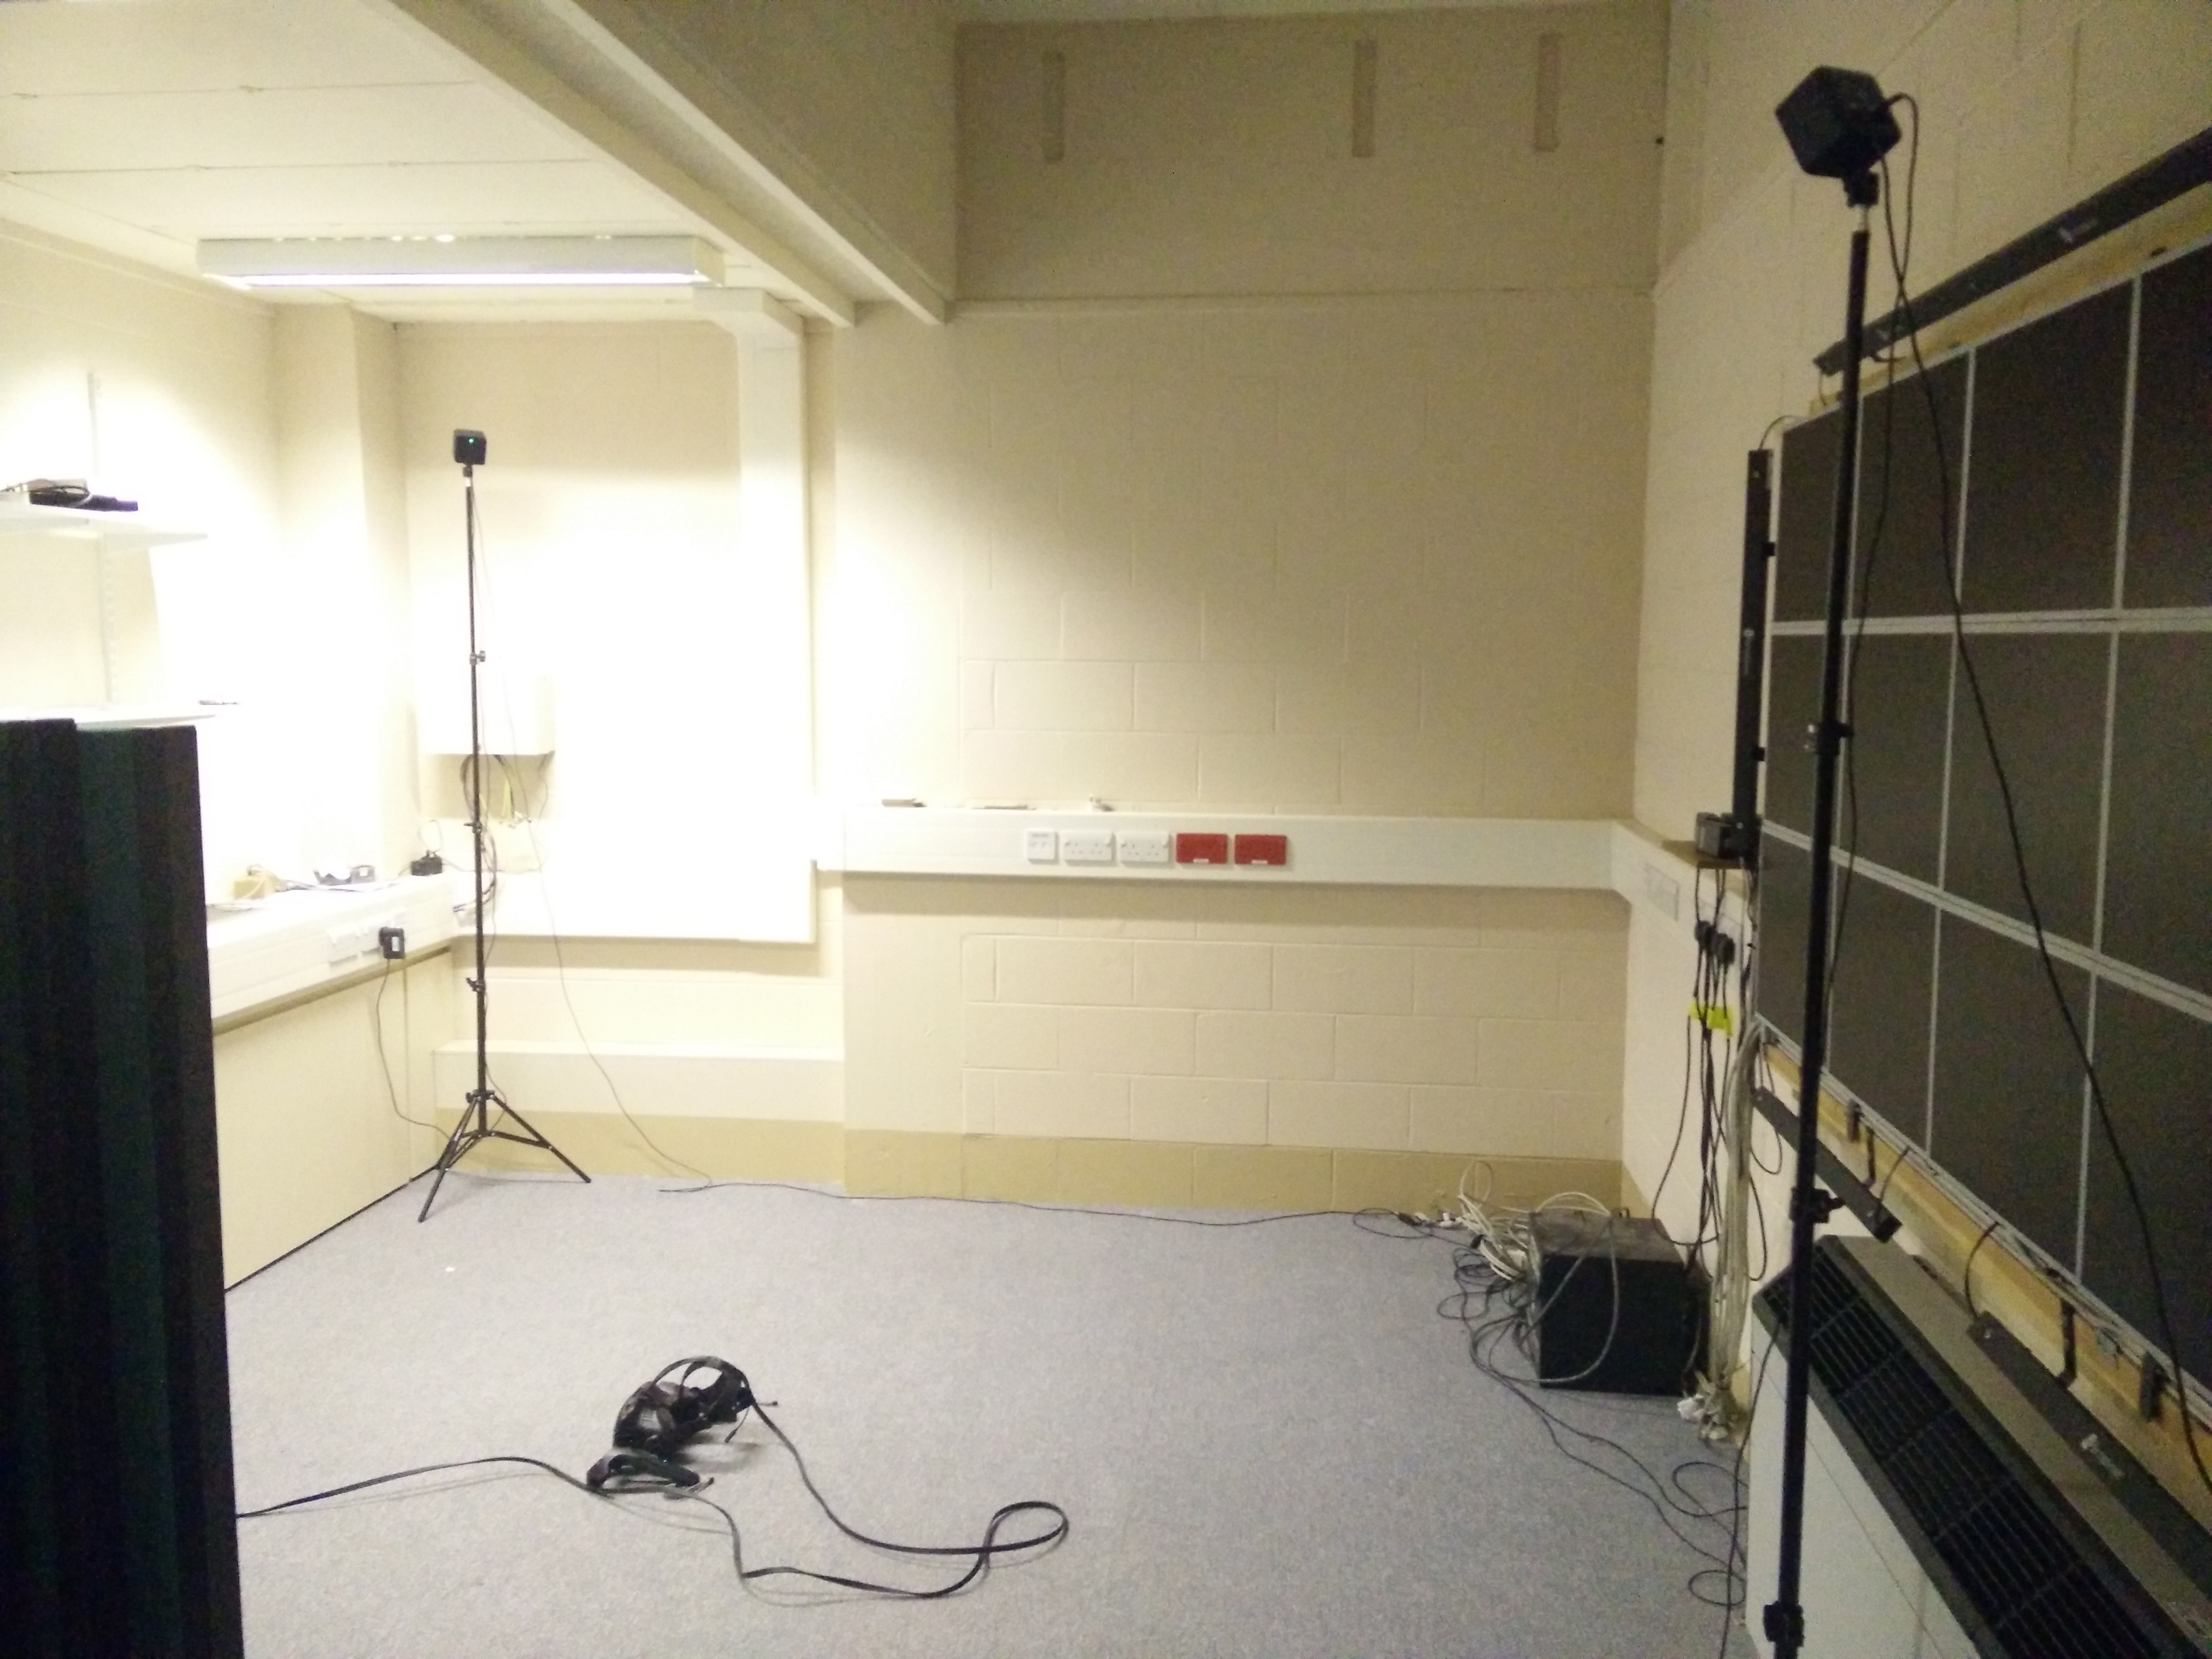
\includegraphics[width=\textwidth]{VRRoom}
	\centering
	\caption{Room used for testing the application}
	\label{fig:VRRoom}
\end{figure}

This room was chosen as it was unused and met the space requirements for the HTC Vive. Approximate room space available resulted in 2.9m x 2.9m which is more than sufficient.

\subsection{Game Engine}
 The chosen game engine used for development as stated in chapter 2 is Unreal Engine. The latest version as of the time of development was used which was Unreal Engine 4.13.2. This decision was made to make sure bugs that may have appeared in previous versions were fixed and also for new features to be taken advantage. Since virtual reality is bleeding edge technology, new features and ways to use VR in development are being implemented rapidly. When development started an older version was being used and new updates were being rolled out, the group decided to update the development environment when a new update was released. It was made sure that everyone in the group was using the same version of Unreal to avoid backward compatibility issues.

\subsection{Visual Studio}
When developing in Unreal Engine, the editor used was Visual Studio. Unreal Engine was designed to integrate smoothly with Visual Studio so code changes can be built in Visual Studio and then can be quickly seen in the Unreal Editor. It also provides a debugging tool to help solve code problems and bugs due to the fact that it has knowledge of the Unreal API. Visual Studio's Intellisense feature has the ability to list members, methods and parameter information when coding. This helped with learning the API, making it easier to detect syntax errors before compiling. The version used was Visual Studio 2015 since Unreal Engine versions 4.10 or later must use this version and not the older 2013 version.

\subsection{Windows}
The operating system used was Windows 10 since the SteamVR software that powers the HTC Vive is only compatible on Windows operating system as of the time of development. Windows 10 was the version that was the latest version and the personal systems the group members owned that were used to develop was already running Windows 10 which made it more convenient to use.

\subsection{Out of Engine Development}
The out of engine development was done in C++, using Sublime Text as an editor, this decision was made out of familiarity with the software. Some C++11 functions and types were used in the development of the graphs, rivers and terrain. The generation for these was done without the use of the Unreal Engine as it outputs files that are then read in with the Unreal code to help generate the game terrain, objects and logic.

\section{Random Generation of Graphs, Rivers and Terrain}

%Divide into sub sections as big topic
\subsection{Graph Generation}\label{subsec:graphGen}
	This section will highlight the main points in the algorithm developed to generate a graph that would be usable by the technology demonstration.

\subsubsection{Start Point Generation}
	The method to generate the starting graph was to start with an empty matrix of nodes, of a size determined by a global variable. These nodes are then all connected using 8-connectedness. This means each node is connected to the eight nodes around it. This makes a graph that looks similar to \ref{fig:triangulation7}.

\begin{figure}[H]
	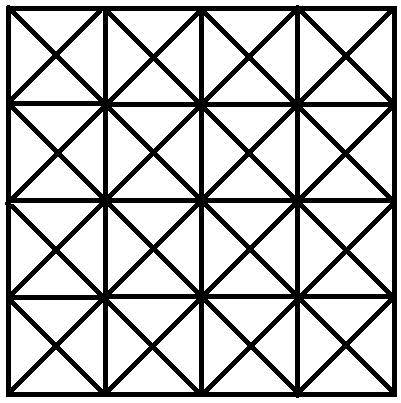
\includegraphics[width=10cm]{triangulation7}
	\centering
	\caption{Image showing an example of the new method of connection the nodes, where the starting matrix is 5 x 5.}
	\label{fig:triangulation7}
\end{figure}

	This produces a connected graph which contains several edges for the connections between nodes to use.\\

\subsubsection{Connections and Weight Matrix}
	The starting set of nodes is found by first selecting the top-left and the bottom-right point as starting nodes, and then randomly selecting others until the amount of nodes selected is the same as the variable stating how many nodes should be selected.
	\newline
	\par
	The weight matrix was made using Manhattan distance between the two connected points as the heuristic. The Manhattan distance is the x distance between the two points plus the distance in the y direction. The Manhattan distance was calculated using the following formula:\\

	$$Manhattan = (point1.x - point2.x) + (point1.y - point2.y)$$
	
	The Manhattan distance then has to be checked to see whether it is positive or not. If it is positive the result is put in element of the matrix representing the first point to the second point, if the result is negative the result is instead placed in the element representing the second point to the first point. This is repeated for each connection in the connection matrix produced before.

\subsubsection{Generating Rivers}
	To generate the rivers the algorithm must first decide which nodes should have rivers running between them. It does this by first finding the distance from the top-left to each of the selected nodes. It then loops through the selected nodes and tries to find two connections where the flow is going downwards. It makes sure the flow is going towards the bottom-right by checking the distances, and if the distance is larger on the node it is trying to connect to, then the river is flowing to the bottom-right. There is a for-loop that will loop through each node, in the order of smallest distance from top-left to largest distance from top-left, looping in this order gives the benefit that the closest nodes to the current will always be selected to connect.\\

	%findConnections code snippet%

	The next step is using Dijkstra's algorithm to find the shortest path between each pair of connected nodes.\\

	%Code snippet for dijkstra's?%

	Using the shortest paths generated by Dijkstra's, a new connection matrix is made. This connection matrix is made by looping through each path made by Dijkstra's algorithm and looking at each pair of nodes. These pairs would be the consecutive nodes in each path. After this connection matrix has been made it is time to map out the graph, so that it can be transferred to the terrain. Mapping out the graph is done by having a matrix of the same size as the terrain will be, this matrix is initialised to have all ones, as the lines will be modify the elements to be 0, as they will be ditches. Then by looping through the connection matrix made before, the connections will be drawn onto the matrix. The connections are drawn onto the matrix by first checking if the element in the connection matrix is 0 or 1, 1 being that there is a connection between the two nodes. If there is a connection then the line between these two points should be drawn onto the height map matrix. This line is calculated by using a modified Bresenham's Line Algorithm, the algorithm is modified so that it can be used in all eight octants of a graph, rather than just the octant that the line goes down and to the right. This modified algorithm is explained in more detail in the section below.

	%Code snippet for drawing lines?%

	The coordinates are then updated so that the coordinates align with the size of the grid, instead of just being consecutive numbers. The coordinate updating is done by first getting the scale factor for the points. The scale factor is the size of terrain divide by the size of the starting matrix, rounded down. The coordinates are then looped over and each x and y coordinate are multiplied by the same scale factor, as the terrain is always square. The last point (the bottom-left point) is then set separately, as it should be set to the bottom-left of the terrain. \\

	%update coordinates code snippet%

	After the coordinates have been updated it is time to generate the connections matrix, this is done by looping over the shortest paths and setting each element in the matrix, that represents the consecutive pairs in the shortest path, to be connected. While the generation code is doing this, it also is determining which nodes should be the "new" nodes. These "new" nodes are where the intersections are in the graph, as the previous nodes are not always guaranteed to be at an intersection. These "new" nodes are used later on in the program in order to decide where to place the rods in the game.
	\newline
	\par
	The program determines which nodes by checking which nodes have been used two times or more. It does this during the for loop when it generates the connection matrix, whenever a element in the connection matrix is set to be connected, then it loops over the array that stores all the connections that have already been used, and checks if the first point of the used connection is the same as the first point in the connection that has just been stored in the connection matrix, it also checks to make sure the second points are different. If the two first points are the same and the two second points are different, then an intersection has been found. The algorithm will then check the array of already found "new" nodes, to make sure that the node doesn't already exist in the array. If it does not exist in the array, it is added to the array, the used connection is then added the array storing all the used connections.\\

	%printGraph snippet%

	After the previous step comes removing edges from the graph that either act as either a sink for the graph, i.e. there are no connections after it, or it acts as a source for the graph, i.e. there are no connections leading to it, as the graph should only have one source, the top-left, and one sink, the bottom-right. The first step in this algorithm is to determine how many times each node has been used as a starting node (being used as the first point in a connection), and how many times it's been used as an end node (being used as the last point in a connection). This is done by looping over the used connections array from the previous step, from each element of this array the start node and end node is extracted. The corresponding nodes then have their respective values incremented in an array for both start nodes and end nodes.
	\newline
	\par
	One of the two cases that are being removed is when a node is not used as an end node, but it is used a start node one or more times. In this case the node would be a source node. This node is then placed in an array of nodes that are removed the graph, and should not be included in it. Now the algorithm needs to look at the nodes that the removed node was connected too, and see if they should be removed. This is done by implementing a stack. The nodes that are connected to the removed node are placed in the stack. This is implemented by having two while loops. One of the while loops is checking to see if the stack is empty, the other is checking if the end of the path has been reached, this being the inner while loop. The end is found when the algorithm can not remove any more nodes from that path. Inside the while loops there is a for loop, looping over the used connections array. For each iteration of this for loop, the start and end node are extracted. The start node is then compared against the node that is being looked at by the algorithm, if they are the same it then checks if there is more than one end node and if the node does not exist in the removed array. If these are both true then the algorithm adds the node to the removed array. The algorithm then needs to find the nodes that are connected to the node that was just removed. The number of connections is found by looping through the connections array and extracting the start node of each element, and incrementing a counter every time the start node matches the removed node. If only one connection is found then the inner while loop carries on, but the current node is now the second point in the connection that was being looked at when the node was removed. If there is more than one connection then every connection found after the first one will have the end node extracted and added to the stack. The end of the inner while loop can also be found if it completes one full cycle of the used connections array without finding any node to remove.
	\newline
	\par
	Once the end of the path has been found, the algorithm will check the size of the stack, if there is nothing inside of the stack, the algorithm will stop. If there is something inside of the stack, the algorithm will use the top value to start its search for nodes to remove, and then remove it from the stack.
	\newline
	\par
	To find the sink nodes the algorithm uses the same method, but instead of using the first node in the connections, it will use the last node of the connections, and whenever the last node was used in this previous part, it will used the first node.
	\newline
	\par
	
	%printGraph snippet%

	The next step of the algorithm is generating the height map for the graph. This is done similarly to the previous method, but with a few notable differences. These differences are in regards to output. In this version of the code, the algorithm needs to output where the rivers and rods are located on the terrain. These are found by first checking if the first node of the connection is a selected node, if it is the line drawing will also record the place that the rod should go. At the first iteration of the line draw algorithm, it records the x and y position of the river for the first side of the river. The x and y coordinates depend on how steep the line is. If the line is 45 degrees or more then the x coordinate is the line's x coordinate plus the river width for one side and minus the river width for the other side. The y coordinate remains the same. If the line is less than 45 degree, then it is the y coordinate which changes with the river width. The same is done for the last iteration of the line draw algorithm. The name of the river is also stored in an array, the name is simply the two nodes that it is connected too. If the line came from a selected node, then a rod needs to be placed. The location of the rod is the same as the line on a set iteration.
	\newline
	\par

	%code snippet%

	After the lines have been drawn, it is time to expand them on the height map, this has to be done so that the connections look more like rivers in the demo. This widening is done by taking a copy of the height map and using the copy to modify the original. The copy of the height map is then looped through, checking each element of the height map. If the original height map is equal to zero, meaning that a line has been drawn in the element, then the algorithm will try to change the value of the pixels in set distance away from this pixel in both the x and y direction, this distance is set as a global variable. The algorithm changes the values of the elements of the copy height map within the range depending on how far away the elements are. Within a third of the distance away the value is set to zero, within two-thirds of the distance then the value is set to $0.33$ and just within the distance it sets the element to $0.66$, this is done as in the game the Towers of Hanoi discs will need to fit inside the rivers, and have their own platform to rest against, and as there are three discs, the distance is split into thirds. The original height map is then replaced by the copy of the height map.
	\newline

	%Code snippet for making ditches

	\par

	The program then needs to recalculate the shortest paths between the nodes, as it needs to output connections between the "new" nodes. This is done using a greedy algorithm, this algorithm will be given a starting river, then in a while loop it will first check if the end node of the river is one of the other "new" nodes, or if the end node is the bottom-right node. If either of these are true, then it will break the while loop. If they are both false, then the greedy algorithm will find the first river that connects to the end node, set the new river as the current river and then the while loop will start again, and it will carry on until it reaches an end node. The algorithm will then return the path it found to the next node.
	\newline
	\par

	%greedy snippet%

	Once all the new shortest paths have been found, these will be output to a file that will be used by the game, so that the game knows the route that the rivers take.\\
	The next step of the program is determining which directions the rivers are flowing into a node, and flowing out of a node. This directions must be found as the game will use this information in order to know where not to place flowers on the terrain. This is done by looping through the new paths and extracting the start and end node from th paths. The algorithm will then search through the array and see if either the start node or the end node is one of the selected nodes. If the node is one of the new selected nodes, then it will check which direction the river came from by comparing the start and end node of the river to each other. As each direction has a distinct amount of difference between them, the direction it is going can be determined. These directions are then output to a file for the game to read in.\\

	%directions snippet%

	At the end of this program the output will look like \ref{fig:triangulation8}

\begin{figure}[H]
	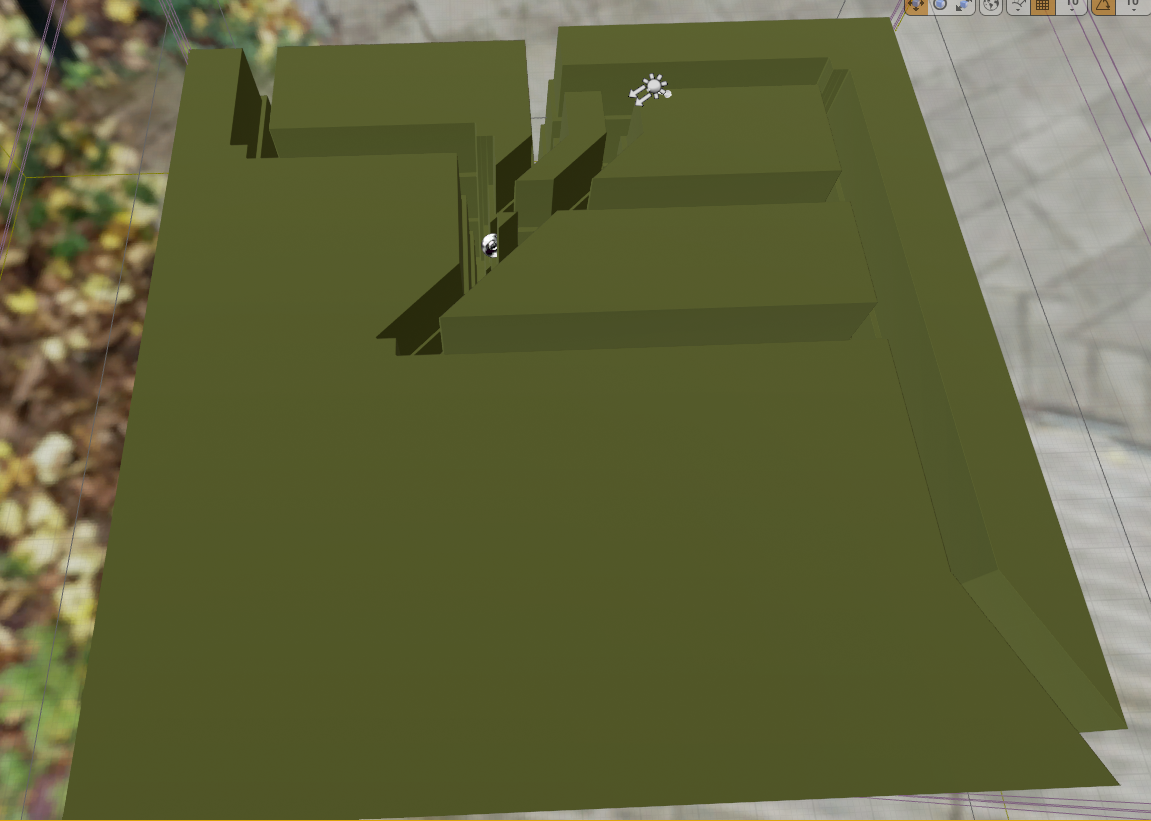
\includegraphics[width=\textwidth]{triangulation8}
	\centering
	\caption{Image showing the output without any randomly generated terrain.}
	\label{fig:triangulation8}
\end{figure}

\subsubsection{Bresenham's Line Algorithm}
	\par
	Bresenham's Line Algorithm is a rasterisation algorithm, it works using error checking for the y coordinate. The original Bresenham's Line algorithm works by finding the absolute value of the gradient, then it loops through each point in the x direction of the line segment. At each iteration through the line it adds the gradient to an error value, when this error value ticks over the value $1$, it will increment the y value of the coordinate for the rest of the iterations. At each iteration of the algorithm, it will plot the point of the current x and y coordinate onto the height map.\\
	The modified Bresenham's Line Algorithm that is used in this project does the same thing, but it lets the algorithm work for lines that are not sloping down and to the right. The modified version does this by first checking the gradient and if the gradient is over $1$ or under $-1$, then the algorithm will swap the x for the y values and the y values for the x values, so that the gradient is less than $1$ and greater than $-1$. The algorithm will then check if the line is sloping to the left or right, the check is comparing the x value of the first point to the x value of the second point and seeing which is bigger. If the line is sloping to the left, the algorithm will swap the points, so that the first point becomes the second point, and the second point becomes the first point. The last step the algorithm takes to ensure that it will work, is that it will check whether the line is sloping upwards, or downwards. If the line is sloping upwards, it will set the change in y to be $-1$, so that it subtracts from the y value, rather than adding it.

	%Code snippet for line drawing%

\subsection{Graph Generation Original Method}\label{subsec:GGOM}
This section will outline some of the previous iterations of the algorithm used to generate graphs, and why these algorithms did not succeed.
\subsubsection{Point Insertion}
\par
	The original idea to do graph generation was to start with a square, using each corner as a node. These nodes would then be connected as shown in \ref{fig:triangulation1}.\\

\begin{figure}[H]
	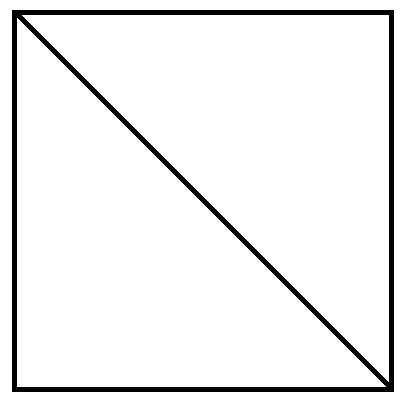
\includegraphics[width=10cm]{triangulation1}
	\centering
	\caption{Original Connections}
	\label{fig:triangulation1}
\end{figure}

	Points would then be inserted into this square, using a random x and y value.  The triangle that this node is in would then be found using the cross product. This was done by checking the cross product of the point and the triangle, for each triangle that is in the graph. The point would then be connected to the corners of this triangle.\\

\begin{figure}[H]
	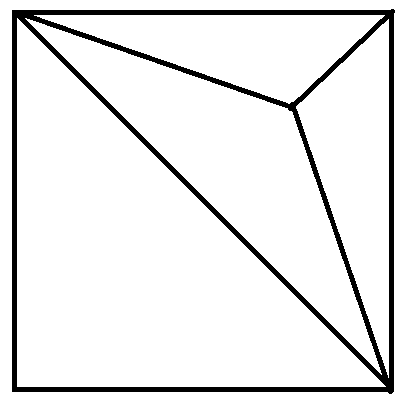
\includegraphics[width=10cm]{triangulation2}
	\centering
	\caption{Example of running the point insertion algorithm for one iteration.}
	\label{fig:triangulation2}
\end{figure}

\begin{figure}[h]
	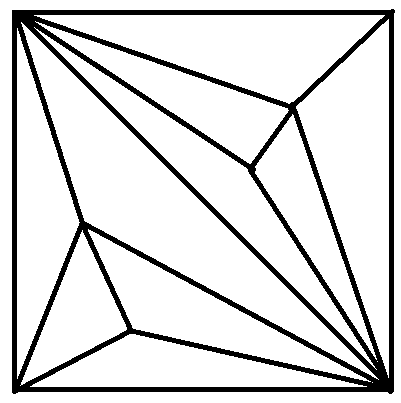
\includegraphics[width=10cm]{triangulation3}
	\centering
	\caption{Example of running the point insertion algorithm for four iterations}
	\label{fig:triangulation3}
\end{figure}

	This approach guaranteed a connected graph to begin with. This approach did not work however as if a node on the bottom-left side of the graph needed to be connected to a node on the top-right side of the graph, the the connection would have to be made through either the top-left node or the bottom-right node, as there was no other way to pass through to the other side of the graph. The approach was then modified slightly to start with an extra node node in the middle of the square, allowing another way to pass through the other side of the graph, this is seen in \ref{fig:triangulation4}.

\begin{figure}[H]
	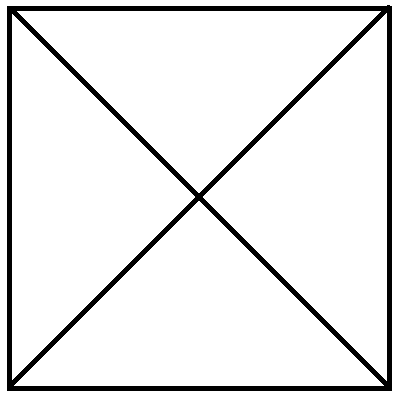
\includegraphics[width=10cm]{triangulation4}
	\centering
	\caption{Image showing the second method's starting connections}
	\label{fig:triangulation4}
\end{figure}
	
	This approach also did not work, as the addition of the extra node did not provide enough of relief for the connections between the two sides of the graph, and the connections would occasionally still go through the top-left or bottom-right node.
The next approach was adding several nodes along the diagonal and connecting them to the corners, similarly to how the middle node was added. The third approach can be seen in \ref{fig:triangulation5}.

\begin{figure}[H]
	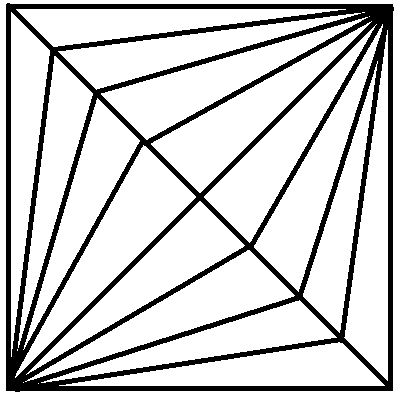
\includegraphics[width=10cm]{triangulation5}
	\centering
	\caption{Image showing the third method's starting connections}
	\label{fig:triangulation5}
\end{figure}
	
	This approach also did not work as when the shortest paths between nodes were found, the paths tended to favour the path from the top-left to the top-right. This would make the graph just be a straight line, with a few edges going to the nodes that were used in the river graph, an example of this can be seen in \ref{fig:triangulation6}.

\begin{figure}[H]
	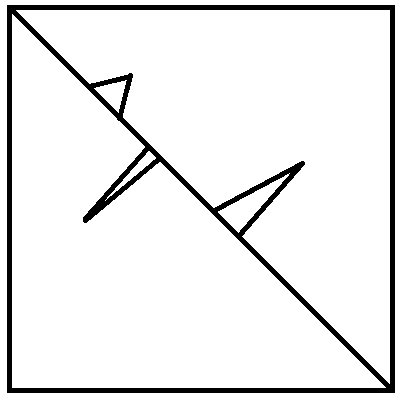
\includegraphics[width=10cm]{triangulation6}
	\centering
	\caption{Image showing an example of the third method's output}
	\label{fig:triangulation6}
\end{figure}

	The next method that was developed was an entire overhaul of the system, and this will be outlined in \ref{subsec:graphGen}



\subsection{Terrain Generation}
	To randomly generate the terrain, the Diamond-square algorithm was used. This algorithm takes four values, to be used as the corners of the terrain, and then generates the rest of the terrain. it does this by alternating between the diamond step and the square step. The algorithm is a recursive algorithm, with each iteration running on a smaller grid.
	\newline
	\par
	The Diamond-square algorithm first takes in an input, which is the size of the step taken in each iteration, to begin with this value is the size of the terrain. This value is halved at each iteration.\\

	%Running code snippet%

	The diamond steps in the algorithm are performed by iterating over all the possible y values in the grid, and at each iteration of that a for loop that iterates over all the possible x points is called. These for loops calculate every possible coordinate to perform the diamond step. The diamond step involves taking four values from the points that are at a distance of the size of the step taken away, and then averaging them and adding a random value. This step is shown in the second step and fourth step of \ref{fig:DiamondSquare}.\\

		%Diamond code snippet%

	The square step is performed by first calculating the possible values of the middle point of the squares. this is done in a for loop as the diamond step was. Then using the calculated coordinates, it will perform the square step on each coordinate. The square step involves taking the points at a distance of the size of the step taken in each of the cardinal directions. these points are then averaged and a random value is added to the value. This value is then placed in the height map at the coordinates that were found before. The square step is shown in the third and fifth step of \ref{fig:DiamondSquare}.

\begin{figure}[H]
	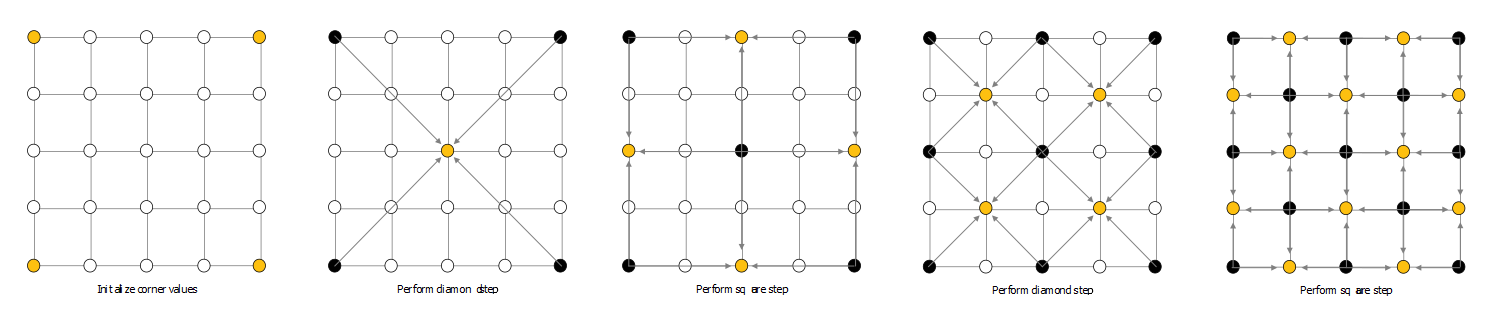
\includegraphics[width=\textwidth]{Diamond_Square}
	\centering
	\caption{Image showing the steps of the Diamond-square algorithm. Image created by Christopher Ewin.}
	\label{fig:DiamondSquare}
\end{figure}

	After the Diamond-square algorithm has been perform and has outputted the height map, the program will then use the heightmap output from the graph generation and the height map from diamond square and combine them into one height map. The equation for doing this is:\\

	$$combinedHeightMap(x, y) =  diamondSquare(x, y) - (0.05 * (1 - graphHeightMap(x, y)))$$

	This formula was determined as the graph height map needs to be subtracted from the diamond square height map in order for the rivers to show up in the terrain. The graph height map is multiplied by $0.05$ so that the rivers are not too deep on the terrain. The graph height map has to be subtracted from one as the rivers in the graph height map have the height 0, and the top of the terrain has the value of 1. This would mean if it is not subtracted from zero, the rivers would show up as mountains on the terrain.\\

\subsection{Final Terrain}
	After these steps have all been performed the program will output the terrain as a model file, as well as many text files including data about where the rivers are, where the rods should be and the route the rivers take. When the model file is imported into the game it looks like \ref{fig:finalTerrain}.

\begin{figure}[H]
	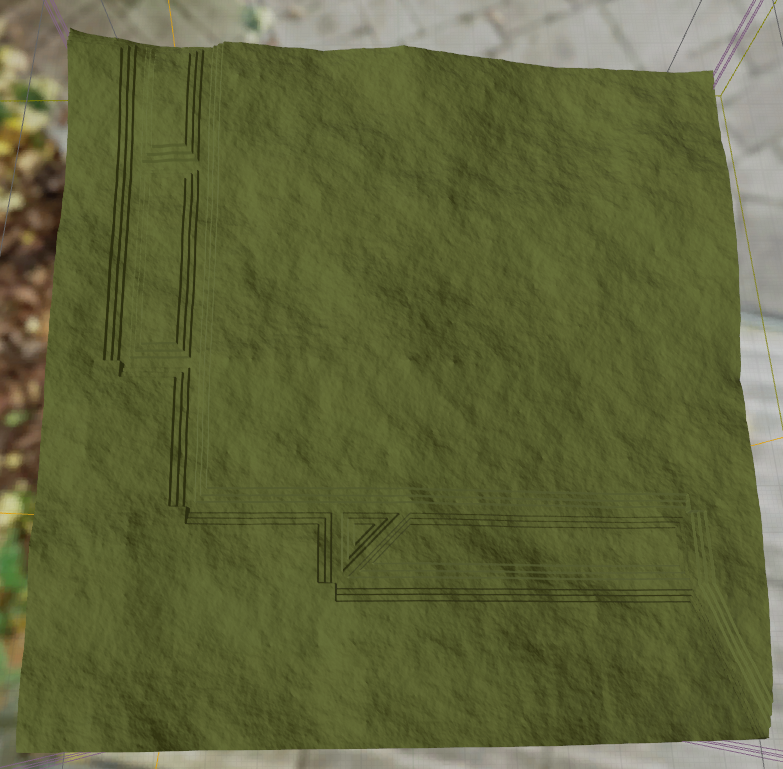
\includegraphics[width=\textwidth]{finalTerrain}
	\centering
	\caption{Image showing the final output of the terrain and river generation.}
	\label{fig:finalTerrain}
\end{figure}


\section{User Interactive Reverse Towers Of Hanoi}
The logic for the reverse Towers of Hanoi was implemented by using collision boxes on the rod actor to act as trigger when Towers of Hanoi discs are placed and removed. This method and actor was used as the basis and control for the Towers of Hanoi logic. To differentiate between the discs, three different actors were created for each size of the Towers of Hanoi discs: small, medium and large. 
\newline
\par
A collision box covers the whole rod with a size that is bigger thane the size of the hole in each disc is set to BlockAll so a disc cannot be placed through the rod. When an actor comes in contact with the collision box, this triggers the rod actor's OnHit collision event. Within this event, it identifies the size of the actor through the name of the actor's class and does a check with the array of discs in which that specific rod currently contains. This simple check will only allow discs which are larger to be placed on top of smaller discs and also makes sure that the array doesn't add disc actors that are already in the array. When the check is passed, the collision box's collision profile name is set to OverlapAll to allow the disc that triggered the event to be placed in that rod otherwise it sets it back to BlockAll. Furthermore, it adds an upward force to the disc to show that the action the player is trying to complete is invalid. This force is only added when the player is not holding the disc to avoid issues when the player is holding the disc and are moving/looking around and accidentally touching a rod with the disc.
\newline
\par
A second collision box that is slightly larger than the first was used to handle the adding and removing of discs to the array which contains all the disc actors which the rod currently holds. When a disc overlaps this collision box it adds it to the array through the OnOverlapBegin event trigger then removes it from the array with the OnOverlapEnd event trigger. When a disc is added to the array, it sets all the discs below it to not allow the player to grab it. This is done to keep with the Towers of Hanoi logic of only the disc at the top of stack being movable.
\newline
\par
A bonus feature to help with placing the discs was implemented with the `snap to rod' feature. When a disc is allowed to be placed on the rod so the disc is larger than the disc below it, then as soon as the OnOverlapBegin collision event is triggered, the disc is teleported to the top of the rod with its rotation reset so it can slide down the rod. This is useful as it can sometimes be bothersome to the player to place the disc exactly so the rod can fit exactly through the hole of the disc. This feature is only in effect when the disc is not currently being held by the player to avoid the disc teleporting whilst the player is still holding the disc which causes the disc to still be attached to the player's hand even though the disc is not in range of the hand's grab sphere.

\section{River Graph Flow}
Graph flow logic was implemented by using information generated with the terrain such as the nodes, IDs of rivers and knowing which rivers are connected to which. An actor for each river is created with a mesh using the UProceduralMeshComponent and the vertices supplied in the rivers.txt file. Each river is given an ID with the first part of the 2 numbers of the ID as the node the river is connected to and the last two numbers as the other node the other end of the river is connected to. This means that a series of river connections have the last two numbers of a river ID identical to the first two numbers of the next river in the connection.
\newline
\par
The river actors are placed in the game world by transforming the coordinates of the vertices for the river mesh generation. Since the coordinate system used for the terrain generation is different to the one used by the Unreal Engine, coordinates produced needs to be transformed so they are correctly placed in the game world as seen in Figure \ref{fig:coordinatesystem}. The X axis is shown in red, Y in green and Z in blue. The top shows the difference in coordinate systems with the coordinate system used to generate the terrain and its output on the left and the Unreal coordinate system on the right. The bottom shows a top view of the terrain ignoring the Z axis since it is the same for both coordinate systems. (0,0) for the terrain file starts at the top left corner where as in Unreal the terrain mesh is placed at the middle of the world at (0, 0, 0). It shows an example of a terrain size used of (1024, 1024) and since the terrain mesh is placed at (0, 0) in Unreal, the centre of terrain becomes (0, 0).
\newline
\par

\begin{figure}[H]
	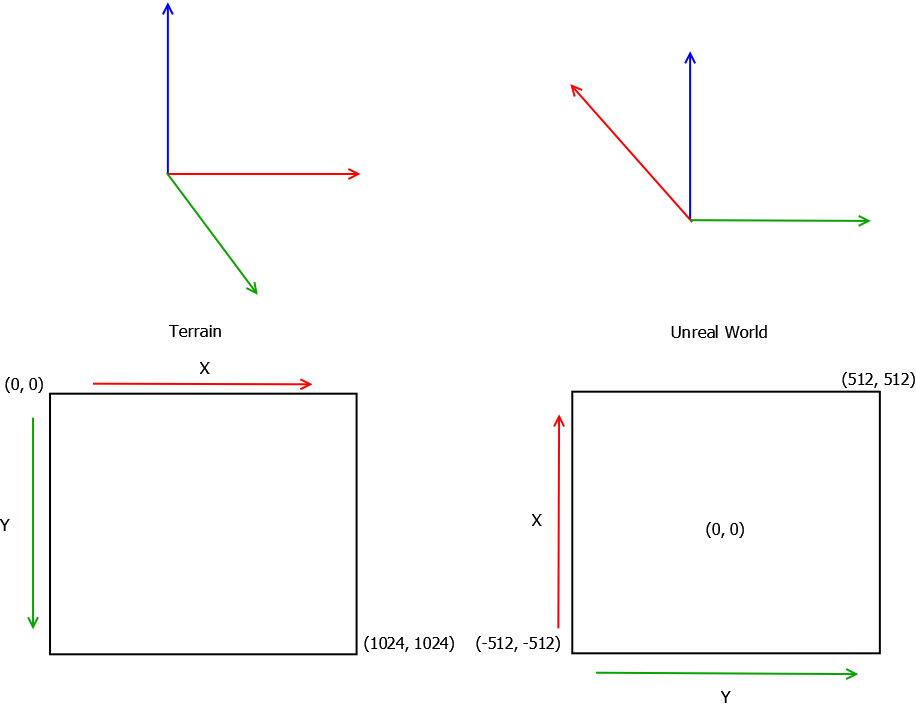
\includegraphics[width=\textwidth]{coordtransform}
	\centering
	\caption{Image showing how terrain coordinates are different to Unreal Engine coordinate system}
	\label{fig:coordinatesystem}
\end{figure}

To calculate the transformation, a bounding box surrounding the terrain mesh is created as seen in Figure \ref{fig:boundingbox}. The vertices of this box is used to compute the scale.
\newline
\par

\begin{figure}[H]
	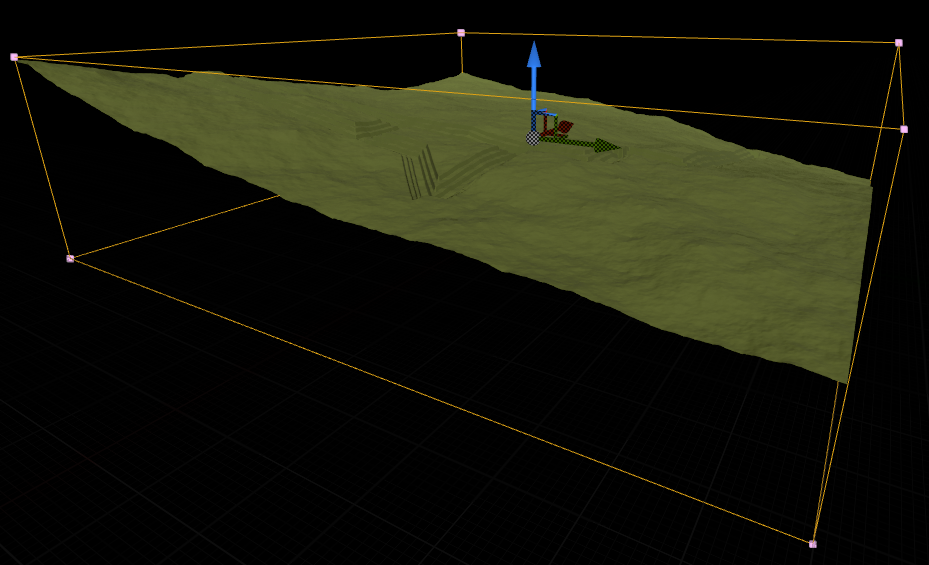
\includegraphics[width=13cm]{bounds}
	\centering
	\caption{Image showing bounding box surrounding terrain mesh}
	\label{fig:boundingbox}
\end{figure}

The following formula is then used for the X and Y coordinates since they are of the same length due to the map being square:
\[transformedCoord = (coord - \frac{1}{2}terrainMax) * \frac{worldCoordMax}{terrainMax}\]

The value of \(coord\) is the coordinate given in the output file from the terrain generation using the origin coordinate system. \(terrainMax\) is the max size of the terrain given by the terrain output so with the example in Figure \ref{fig:coordinatesystem}, this would be 1024. Half of this is subtracted as the offset to make the coordinate in the same position but instead in the bottom left corner instead of top left to fit with the coordinate system. Now this is scaled by computing the scale factor using the bounding box coordinate of a vertex but doubled as \(worldCoordMax\) to get the length of X (Y is the same) divided by \(terrainMax\).
\newline
\par
The Z transformation is similar but the only transformation needed is a scale which is just the height of the bounding box. This is computed by subtracting the Z coordinate of an upper corner of a bounding box with the Z coordinate of a lower corner. The \(terrainMax\) is not used because it would always be 1 since the Z coordinates of the terrain are between 1 and 0 with 1 as the highest point and 0 as the lowest.
\newline
\par
This method is then used to place the rods in their right places in the world so where there is a split in a river, a rod is placed on each of the rivers that branch out. The position of the rods are read in through the rods.txt file output from the terrain generation process. Each rod is given information regarding its own node ID and the river actor which it is connected to.
\newline
\par
The source of the river in the graph has a flow value hard coded and then iterates through its river connection changing the flow value of each river then when it reaches the final river it means that the river has reached a node where it splits in to two. This split has a rod for each river in order for the player to change the flow of each river. With rods with no discs, the flow value is just split simply in half between the two rivers which then follows the same procedure as before and changes the flow value of the rivers in its river connections.
\newline
\par
With the case of rods with discs in them, the flow is then affected depending on which discs are used. A small disc will reduce the flow value of the river by a \(\frac{1}{6}\), medium disc by \(\frac{1}{3}\) and a large disc by \(\frac{1}{2}\). This means using all three discs would reduce the flow to 0 so completely blocking it off. Adding or removing a disc from a rod would change the flow value for the river the rod is connected to which then changes the flow value of all the rivers that this river affects.
\newline
\par
In order for the player to easily distinguish a difference in the flow of a river when changing them with the discs, the opacity of the material used on the river will change depending on the flow value as a percentage of the original flow value at the source.

\section{Flow Dependant Flora}
Flower models are spawned around each of the nodes with rods. Flower model is royalty free and taken from cgtrader\cite{flowermodel}. The first node with rods do not have flowers as the flows of the river that will act as input to this node are the same value as the flow at the source due to the fact that it has yet to be split. These flowers will act as indicators to the player whether or not they are getting closer to the goal.
\newline
\par
The position of the flower models are computed by using the coordinates of the nodes found in the nodes.txt file output through the terrain generation procedure. The coordinates are then transformed to be placed correctly in the world with the same process as before. Another file is used called nodeConnections.txt which shows information on directions of the rivers that node is connected to. This is used to place the flowers in places on the terrain where there is no river. Due to method used to generate the terrain a river can go in one direction out of a possible 8. These possible directions can be described using the points in a compass e.g. North, North-East, East and so forth. Using random number generation, a flower has a one in three chance of placing a flower on a free space but makes sure at least one flower is placed for each node.
\newline
\par
When the player places a disc on a rod and changes the flow of the corresponding river and all the rivers affected by the change, all the river flows that serve as input in a node are accumulated and checks against the required flow to complete the goal for the node. If the flow value is over the required flow, the material for the flower petals are changed to a blue colour. If the flow value is lower than the required flow, the petals then change to a white colour. When the required flow is met, the colour is changed to an orange colour. This visual indicator helps the player see their current progress and helps to solve the puzzle.

\section{Game Goal Computation}
In order for the game to provide a challenge to players such as University of Leeds applicants during applicant days, there needs to be a goal or a puzzle to be solved. The goal is implemented using random generation every time the terrain class is added in to the Unreal Editor scene. This randomness is controlled by limiting it to only possible solutions and this is done through simulation of the game before it is created.
\newline
\par
For each rod actor in the map, one of the many possible disc combinations is chosen out of random which includes no disc on that rod. Then the game is simulated with the river flow values which are then affected by the discs on each rod. The flow value for all the rivers that act as input to the ndoes are then accumulated and is saved as the required flow for that node. The simulation is ended and resets the game with no discs on every rod then resets all the flow values to be computed again. The player will then need to try figure out the correct disc combinations for each rod through trial and error to meet all the required flows for each node to make the flower petals turn to orange which means the goal has been met. When all flowers turn to orange, the level puzzle is completed so the game transports the player to the next level.

\section{Sky Textures}
The textures for the three levels are from various places around the University of Leeds, level 1 is from in front of the Roger Stevens Building \ref{fig:level3Backdrop}, level 2 is from in front of the Great Hall \ref{fig:level2backdrop}, and level 3 is from in front of the union \ref{fig:level3Backdrop}. This was done to show that the project was developed in the University.

%Insert Images from each level showing backdrops%
\begin{figure}[H]
	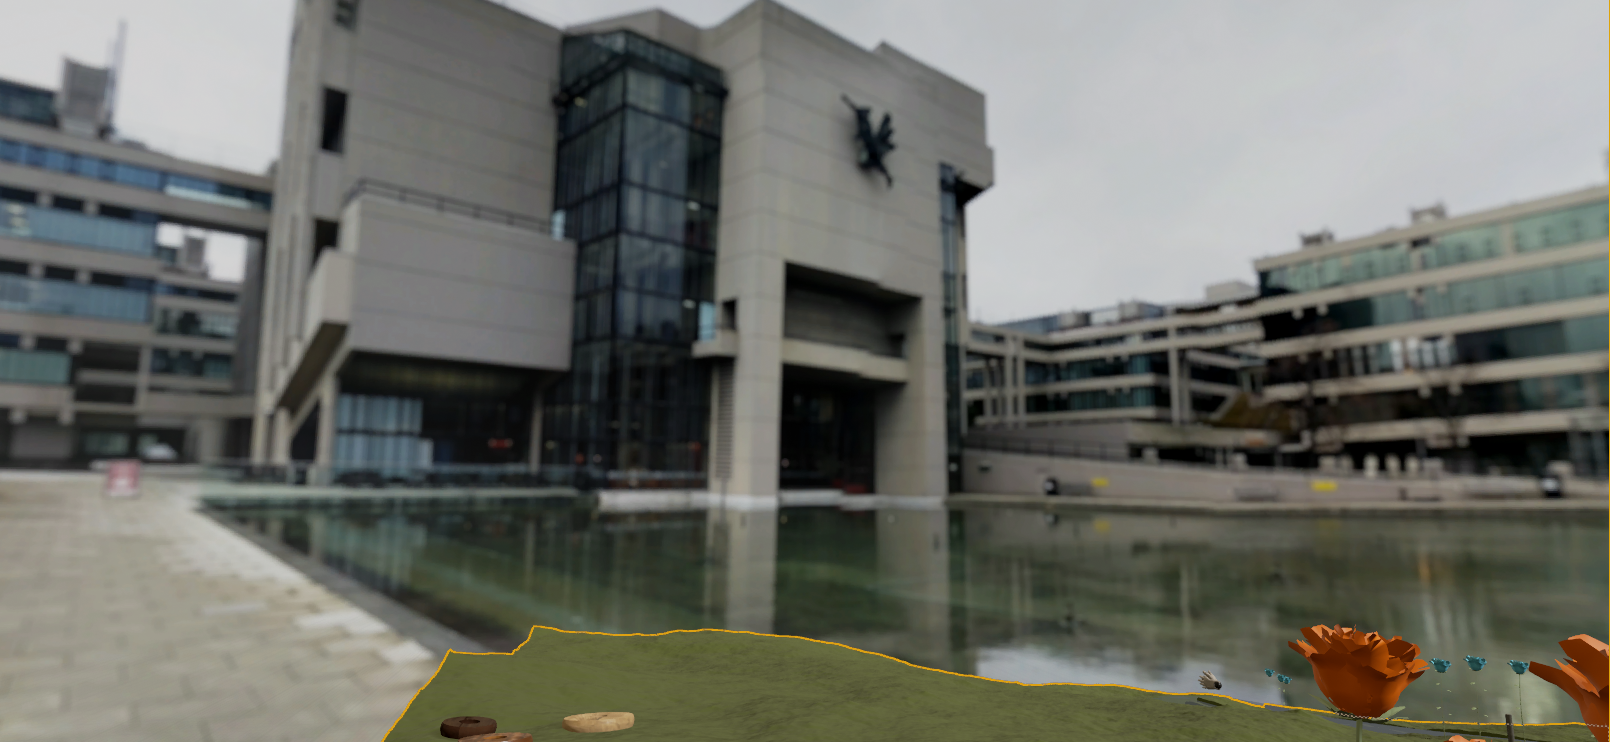
\includegraphics[width=13cm]{level1Backdrop}
	\centering
	\caption{Image showing the Sky Texture on level 2}
	\label{fig:level1Backdrop}
\end{figure}

\begin{figure}[H]
	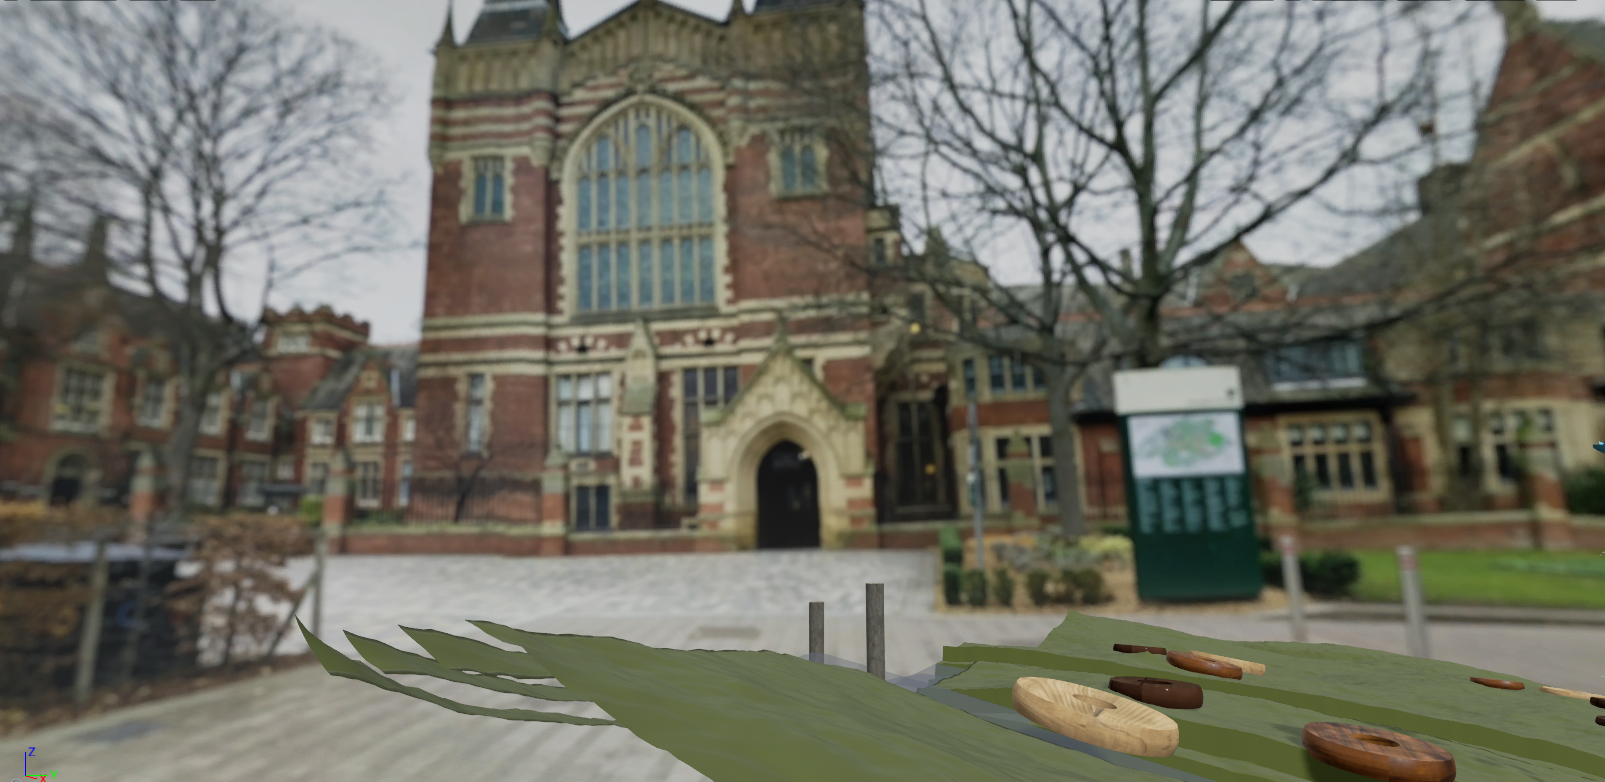
\includegraphics[width=13cm]{level2Backdrop}
	\centering
	\caption{Image showing the Sky Texture on level 2}
	\label{fig:level2Backdrop}
\end{figure}

\begin{figure}[H]
	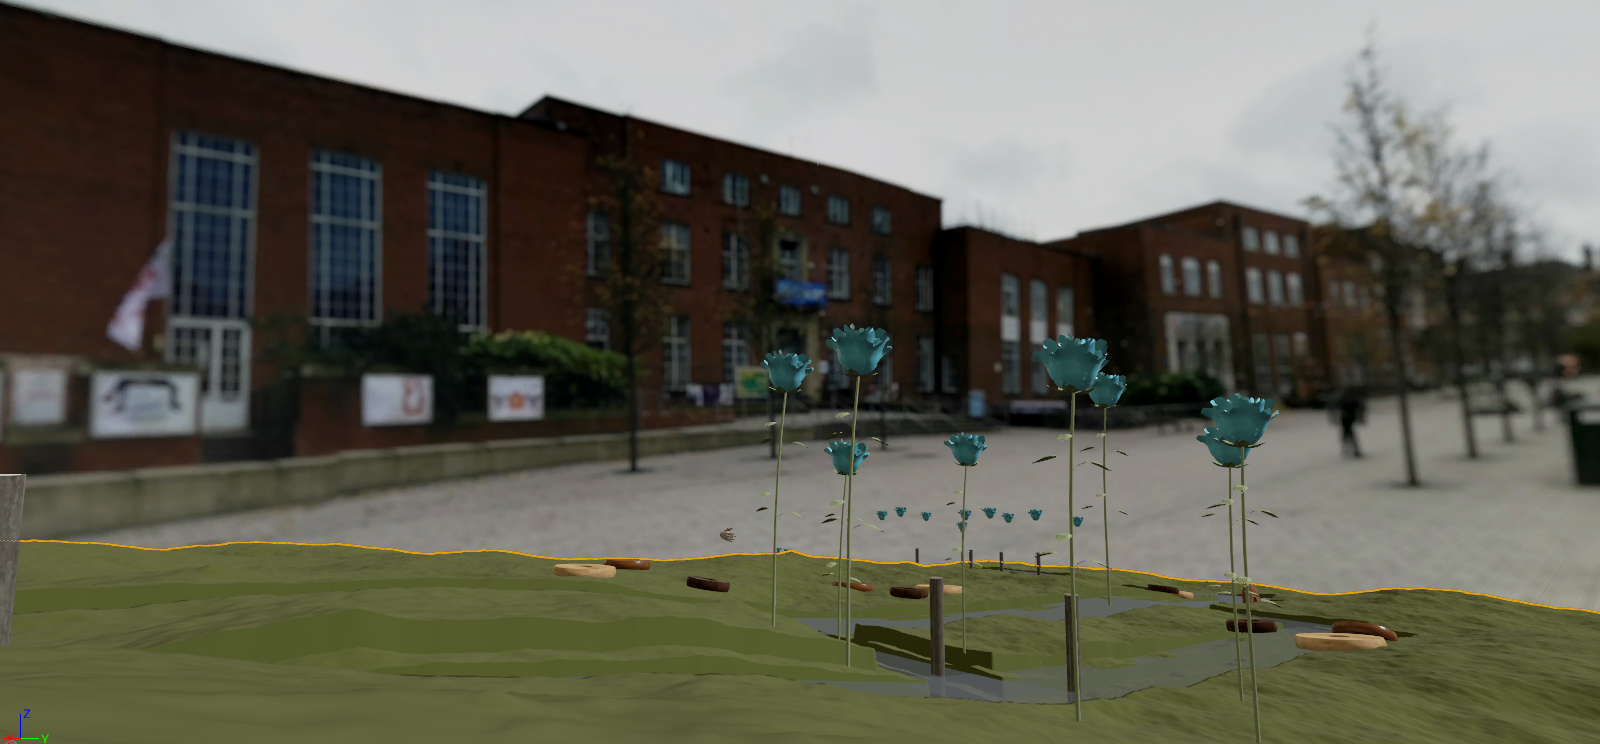
\includegraphics[width=13cm]{level3Backdrop}
	\centering
	\caption{Image showing the Sky Texture on level 2}
	\label{fig:level3Backdrop}
\end{figure}

These textures were made by first using Google's Photosphere software to create a 360 degree image of the location, this image was then flipped horizontally so that they would appear the correct way in the game. These are shown in \ref{fig:rogerStevens}, \ref{fig:greatHall}, and \ref{fig:union}. 

\begin{figure}[H]
	\includegraphics[width=13cm]{RogerStevens}
	\centering
	\caption{Image showing the 360 degree image by the Roger Stevens Building}
	\label{fig:rogerStevens}
\end{figure}

\begin{figure}[H]
	\includegraphics[width=13cm]{GreatHall}
	\centering
	\caption{Image showing the 360 degree image by the Great Hall}
	\label{fig:greatHall}
\end{figure}

\begin{figure}[H]
	\includegraphics[width=13cm]{Union}
	\centering
	\caption{Image showing the 360 degree image by the Student Union}
	\label{fig:union}
\end{figure}

These images were then separated into six images using a blender file obtained from "Aerotwist.com" \cite{aerotwist}. Using these separate images they were then arranged in the order specified by Unreal in order to create a cube map using the nVidia Texture Tools \cite{unrealCubeMaps}, an example of the image ready to be exported by nVidia texture tools is shown in \ref{greatHallPre}.

\begin{figure}[H]
	\includegraphics[width=13cm]{GreatHallPre}
	\centering
	\caption{Image showing an image about to be exported by nVidia texture tools}
	\label{fig:greatHallPre}
\end{figure}

This image is then processed by nVidia Texture Tools and exported as a .dds file, a file type that is supported by Unreal Engine. This file is then imported into the Unreal project and a material is created from the file. This material is then modified slightly so that it works as a spherical texture, and then it is set as the texture for the Sky Sphere.

\section{Disc Respawning}
An issue that was found during testing was that the discs could easily fall off the terrain. This was solved by placing invisible walls around the terrain, which stopped the discs from flying off of the edge of the terrain as they would just bounce off the wall. This wall could not be too close to the terrain however, as sometimes the discs would need to be placed on the edges of the terrain as a rod would be close to the edge of the terrain. This meant in addition to the invisible wall around the terrain, a trigger box had to be added underneath the terrain. A trigger box is an object in the world that when an object collides with it, it produces a collision event on the object. This was used by the discs, if the discs had a collision event caused by the trigger box, the discs would return to their original spawning location. this solved the issue of discs falling off the edge and not being to retrieve them.